% =====================================================================
%  model_architecture.tex
%
%  Architecture and pipeline reference for the PJM zonal load-forecasting
%  repository (pjm_load_xgboost).  Every dimension, layer and equation in
%  this document was read off the source; the file/line pointers in the
%  margin notes say where.
%
%  Compile:  pdflatex model_architecture.tex   (twice, for the ToC)
%  Needs:    amsmath, amssymb, booktabs, geometry, tikz, xcolor, hyperref
% =====================================================================
\documentclass[11pt]{article}

\usepackage[utf8]{inputenc}
\usepackage[T1]{fontenc}
\usepackage{amsmath,amssymb,amsfonts}
\usepackage{booktabs}
\usepackage{array}
\usepackage{longtable}
\usepackage{multirow}
\usepackage[margin=1in]{geometry}
\usepackage{xcolor}
\usepackage{tikz}
\usetikzlibrary{arrows.meta,positioning,fit,calc,shapes.geometric,backgrounds}
\usepackage[hidelinks]{hyperref}
\usepackage{microtype}
\usepackage{caption}

% Shrink a diagram only if it would overflow the text block; leave it alone
% otherwise. graphicx is already loaded by tikz.
\newcommand{\fitfig}[1]{%
  \resizebox{\ifdim\width>\linewidth \linewidth\else \width\fi}{!}{#1}}

% --- notation shorthands ------------------------------------------------
\newcommand{\R}{\mathbb{R}}
\newcommand{\E}{\mathbb{E}}
\newcommand{\Prob}{\mathbb{P}}
\newcommand{\Loss}{\mathcal{L}}
\newcommand{\Hset}{\mathcal{H}}
\newcommand{\code}[1]{\texttt{\small #1}}
\newcommand{\dims}[1]{\ensuremath{\left(#1\right)}}
\newcommand{\LN}{\mathrm{LayerNorm}}
\newcommand{\MHA}{\mathrm{MHA}}
\newcommand{\FFN}{\mathrm{FFN}}
\newcommand{\ReLU}{\mathrm{ReLU}}
\newcommand{\PReLU}{\mathrm{PReLU}}
\newcommand{\softmax}{\mathrm{softmax}}
\newcommand{\Drop}{\mathrm{Dropout}}
\newcommand{\ind}{\mathbf{1}}
\newcommand{\note}[1]{\marginpar{\raggedright\scriptsize\color{gray}#1}}

% --- TikZ styles --------------------------------------------------------
\tikzset{
  blk/.style   ={draw, rounded corners=2pt, align=center, font=\small,
                 minimum height=8mm, inner sep=3pt, fill=blue!4},
  data/.style  ={draw, align=center, font=\small\ttfamily,
                 minimum height=7mm, inner sep=3pt, fill=gray!8},
  op/.style    ={draw, rounded corners=6pt, align=center, font=\small,
                 minimum height=8mm, inner sep=3pt, fill=orange!10},
  dim/.style   ={font=\scriptsize\ttfamily, color=blue!55!black},
  ar/.style    ={-{Latex[length=2mm]}, thick},
  ard/.style   ={-{Latex[length=2mm]}, thick, dashed, color=gray!70!black},
}

\title{PJM zonal load forecasting: features and model structures}
\author{}
\date{}

\begin{document}
\maketitle
\vspace{-3em}

\noindent
Record of what goes into the models and what they are. One dataset (PJM zone
\code{dom} or \code{bge}), nine point architectures $\times$ \{direct, residual\},
four probabilistic baselines. TimesFM is excluded --- pre-trained elsewhere.
Numbers are \code{dom}, arm \code{\_cong}, unless said otherwise.

% =====================================================================
\section{Dataset and features}
% =====================================================================

\noindent
Sources: PJM Dataminer2 (metered + preliminary load, Day-Ahead marginal value,
zonal LMP) and Open-Meteo (ERA5 observed weather, forecast archive). Merged on
the UTC hour into \code{cleaned\_pjm\_load\_weather.csv} ($49\,511$ rows); the
weather-forecast, congestion and Day-Ahead price tables stay on their own index
because they are looked up per \emph{target day}, not per row.

\subsection{The task and the blind spot}

Given everything known at midnight EPT on day $d$, forecast the 24 hourly loads
of day $d{+}1$. Day $d$ itself is never observed.

\begin{figure}[htbp]
\centering
\fitfig{%
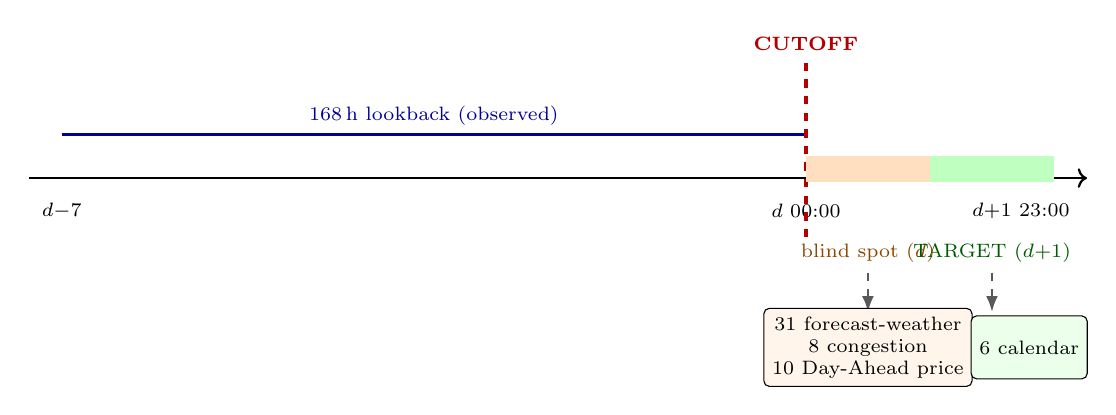
\begin{tikzpicture}[x=1.05cm,y=1cm]
\draw[thick,->] (-0.4,0) -- (12.4,0);
\node[font=\scriptsize] at (0,-0.42)    {$d{-}7$};
\node[font=\scriptsize] at (9,-0.42)    {$d$ 00:00};
\node[font=\scriptsize] at (11.6,-0.42) {$d{+}1$ 23:00};
\draw[very thick, blue!60!black] (0,0.55) -- (9,0.55);
\node[font=\scriptsize,blue!60!black,above] at (4.5,0.55) {168\,h lookback (observed)};
\draw[very thick, red!70!black, dashed] (9,-0.75) -- (9,1.5);
\node[font=\scriptsize\bfseries, red!70!black, above] at (9,1.5) {CUTOFF};
\fill[orange!25] (9,-0.05) rectangle (10.5,0.28);
\node[font=\scriptsize, orange!55!black] at (9.75,-0.95) {blind spot ($d$)};
\fill[green!25] (10.5,-0.05) rectangle (12,0.28);
\node[font=\scriptsize, green!35!black] at (11.25,-0.95) {TARGET ($d{+}1$)};
\draw[ard] (9.75,-1.2) -- (9.75,-1.7);
\node[blk, font=\scriptsize, fill=orange!8] at (9.75,-2.15)
  {31 forecast-weather\\8 congestion\\10 Day-Ahead price};
\draw[ard] (11.25,-1.2) -- (11.25,-1.7);
\node[blk, font=\scriptsize, fill=green!8] at (11.7,-2.15) {6 calendar};
\end{tikzpicture}}
\caption{Three static blocks exist specifically to describe the blind-spot day.
All are known before the cutoff: day $d$'s Day-Ahead market clears $\approx$13:30
on $d{-}1$, and the 48\,h weather forecast covering $d$ and $d{+}1$ is issued on
$d{-}2$. A target day missing either is dropped from the matrix, not zero-filled.}
\end{figure}

\subsection{Sequence channels --- $C_{\text{seq}} = 22$, or $25$ with prices}

One value per hour, fed to the encoder as a $(168, C_{\text{seq}})$ series.

\begin{center}\small
\begin{tabular}{@{}llp{8.4cm}@{}}
\toprule
Group & \# & Columns \\
\midrule
Load & 1 & \code{Load\_Estimated} (preliminary, published in real time) \\
Weather & 11 & \code{Temp\_F}, \code{ApparentTemp\_F}, \code{Dewpoint\_F},
  \code{RelativeHumidity\_pct}, \code{SolarRadiation\_Wm2}, \code{WindSpeed\_mph},
  \code{WindDirection\_deg}, \code{WindGusts\_mph}, \code{Precip\_in},
  \code{CloudCover\_pct}, \code{SoilTemp0\_7cm\_F} \\
Thermal & 10 & \code{CDD\_h}, \code{HDD\_h}, \code{CDD\_cum\_\{24,48,72\}h},
  \code{Temp\_ma\_\{24,72\}h}, \code{Temp\_delta\_24h}, \code{HeatIndex\_F},
  \code{WetBulb\_F} \\
RT price & 3 & \code{RT\_\{Total,Energy,Cong\}\_slog} \hfill (\code{PJM\_LMP=1} only) \\
\bottomrule
\end{tabular}
\end{center}

\noindent
With $T_b = 65^\circ$F: $\mathrm{CDD}_t = \max(0, T_t - T_b)$,
$\mathrm{HDD}_t = \max(0, T_b - T_t)$, rolling sums/means strictly causal,
$\Delta T_t = T_t - T_{t-24}$. Heat index is the NWS Rothfusz regression,
wet bulb the Stull (2011) approximation.

\noindent
Prices use a signed log, $\mathrm{slog}(x) = \operatorname{sign}(x)\log(1+|x|)$:
RT LMP has a $120\times$ right tail and is negative in ${\approx}22\%$ of hours,
so \code{log1p} is undefined and a raw channel is flattened by standardisation.

\subsection{Static features --- one value per sample, $S = 40/48/50/58$}

Broadcast across the window in storage, but every neural model slices them back
out at $t=0$ and concatenates them \emph{after} the encoder, so the encoder never
re-reads a constant 168 times.

\begin{center}\small
\begin{tabular}{@{}llp{8.6cm}@{}}
\toprule
Block & \# & Content \\
\midrule
Calendar & 6 & of the \emph{target} day: $\sin/\cos$ month, $\sin/\cos$ day-of-week,
  \code{is\_weekend}, \code{is\_holiday}. Hour-of-day is absent --- implicit in the
  24-dim output \\
Macro & 4 & 3-week context from \emph{preliminary} load: two night-load $q_{05}$
  week-over-week slopes, a 2-week energy ratio, and the mean $|{\cdot}|$ error of a
  168\,h-lag naive forecast over the last 6 hours \\
Thermal state & 5 & yesterday's max temp and CDD total, 3-day max temp, CDD ratio
  (day$_1$/day$_2$, ${>}1$ when heat is building), 3-day mean-temp change \\
Forecast weather & 31 & 24 per-hour departures $\hat T^{(1)}_h - r_h$ ($r_h$ = mean
  observed temp at clock hour $h$ over the window), 5 CDD/HDD/max departures,
  2 absolute anchors (day-$d{+}1$ max and 14--19\,h mean) \\
Congestion & 8 & RTO-wide DA shadow prices on day $d$, as departures from trailing
  3/7/21-day means; one level form kept \hfill (\code{PJM\_CONGESTION=1}) \\
DA price & 10 & day-$d$ DA energy / zonal spread / total, same departure form
  \hfill (\code{PJM\_LMP=1}) \\
\bottomrule
\end{tabular}
\end{center}

\noindent
Departures, not levels, almost everywhere: 168 hours of observed temperature
already state the level. A LightGBM gain breakdown put the congestion departure
at $3.31\%$ of total gain and the same quantity as a level at $0.06\%$.
The three absolute anchors survive because load responds non-linearly to
temperature --- $+8^\circ$F on a $92^\circ$F base is worth far more MW than on
$62^\circ$F.

\subsection{The two matrices, and the four arms}

\begin{center}\small
\begin{tabular}{@{}lrrrrrr@{}}
\toprule
Arm (\code{MATRIX\_TAG}) & $C_{\text{seq}}$ & cal & $S$ & $C$ & \code{X\_3d} & \code{X\_opt} cols \\
\midrule
\code{''} \hfill (cong 0, lmp 0) & 22 & 6 & 40 & 68 & $(1957,168,68)$ & 3742 \\
\code{\_cong} \hfill (1, 0)      & 22 & 6 & 48 & 76 & $(1957,168,76)$ & 3750 \\
\code{\_lmp} \hfill (0, 1)       & 25 & 6 & 50 & 81 & $(1957,168,81)$ & 4256 \\
\code{\_cong\_lmp} \hfill (1, 1) & 25 & 6 & 58 & 89 & $(1957,168,89)$ & 4264 \\
\bottomrule
\end{tabular}
\end{center}

\noindent
\textbf{3-D tensor} (sequence models): standardised series $\Vert$ calendar
$\Vert$ standardised statics, the last two broadcast over $t$.
\textbf{2-D matrix} (trees): the window flattened column-wise into
\code{\{channel\}\_h\{k\}}, $k=0$ oldest, values raw --- trees are invariant to
monotone rescaling. Three scalers are fit on the leading $84\%$ and persisted, so
the test period never touches them.

\noindent
Every target day is coerced to exactly 24 EPT slots: a 25-hour DST day averages
the repeated hour, a 23-hour day interpolates the missing one. Without this
\code{out\_dim}$=24$ would be wrong twice a year.

\subsection{Split}

Chronological tail split on the $N = 1957$ daily samples:

\begin{center}\small
\begin{tabular}{@{}lrl@{}}
\toprule
Block & $n$ & Rule \\
\midrule
train & $1466 \to \mathbf{1461}$ & the rest; then drop days with any 3-sigma outlier or unlabelled hour \\
--- embargo & $14$ d & macro features look back 504\,h, so without it a training sample's own window overlaps val \\
val   & $\mathbf{150}$ & last $10\%$ of the training pool, minus the embargo \\
--- embargo & $14$ d & \\
test  & $\mathbf{313}$ & last $\lfloor 0.16N \rfloor$ days, never trimmed, mask never applied \\
\bottomrule
\end{tabular}
\end{center}

\noindent
Tree models have no validation block, so their run tag is \code{tail\_test0.16}
against the sequence models' \code{tail\_test0.16\_tail\_val0.1}; both then carry
the arm tag.

% =====================================================================
\section{Point models}
% =====================================================================

\noindent
Every model emits $\hat{\mathbf{y}} \in \R^{B\times24}$ in standardised target
space; the evaluator applies $\hat y^{\text{MW}} = \sigma_y \hat y + \mu_y$ once.
Trees are the exception --- fit on raw MW.

\noindent
\textbf{Neural training} (all but GARCHFormer): Huber $\delta=1$ on standardised
targets, AdamW $3{\cdot}10^{-4}$ (LSTM $10^{-3}$), weight decay $10^{-4}$, batch 32,
grad-norm clip 1.0, \code{ReduceLROnPlateau}$(\times0.5$, patience 10$)$, early
stop patience 50, max 200 epochs, best-validation checkpoint kept.

\subsection{Trees --- XGBoost, LightGBM}

No single model: each of the 24 target hours gets its own regressor on the same
$(B, 3750)$ matrix.
\[
\hat y_{i,h} = F_h(\mathbf{x}_i) = \sum_{m=1}^{1000}\eta\,f_{h,m}(\mathbf{x}_i),
\qquad h = 0,\ldots,23,\quad \mathrm{depth}(f) \le 3 .
\]
So a saved model is 24 boosters, $24\,000$ trees. Nothing ties the 24 outputs
together, which is why tree profiles are visibly rougher than sequence ones.
XGBoost: $\eta = 0.01277$, $\lambda = 9.34$, $\alpha = 0.51$, row/col subsample
$0.87/0.73$, level-wise. LightGBM: $\eta = 0.00755$, $\lambda = 1.40$,
$\alpha = 0.001$, $0.70/0.74$, \code{min\_child\_samples} 40, leaf-wise.

\subsection{Transformer}\label{sec:transformer}

\begin{figure}[htbp]
\centering
\fitfig{%
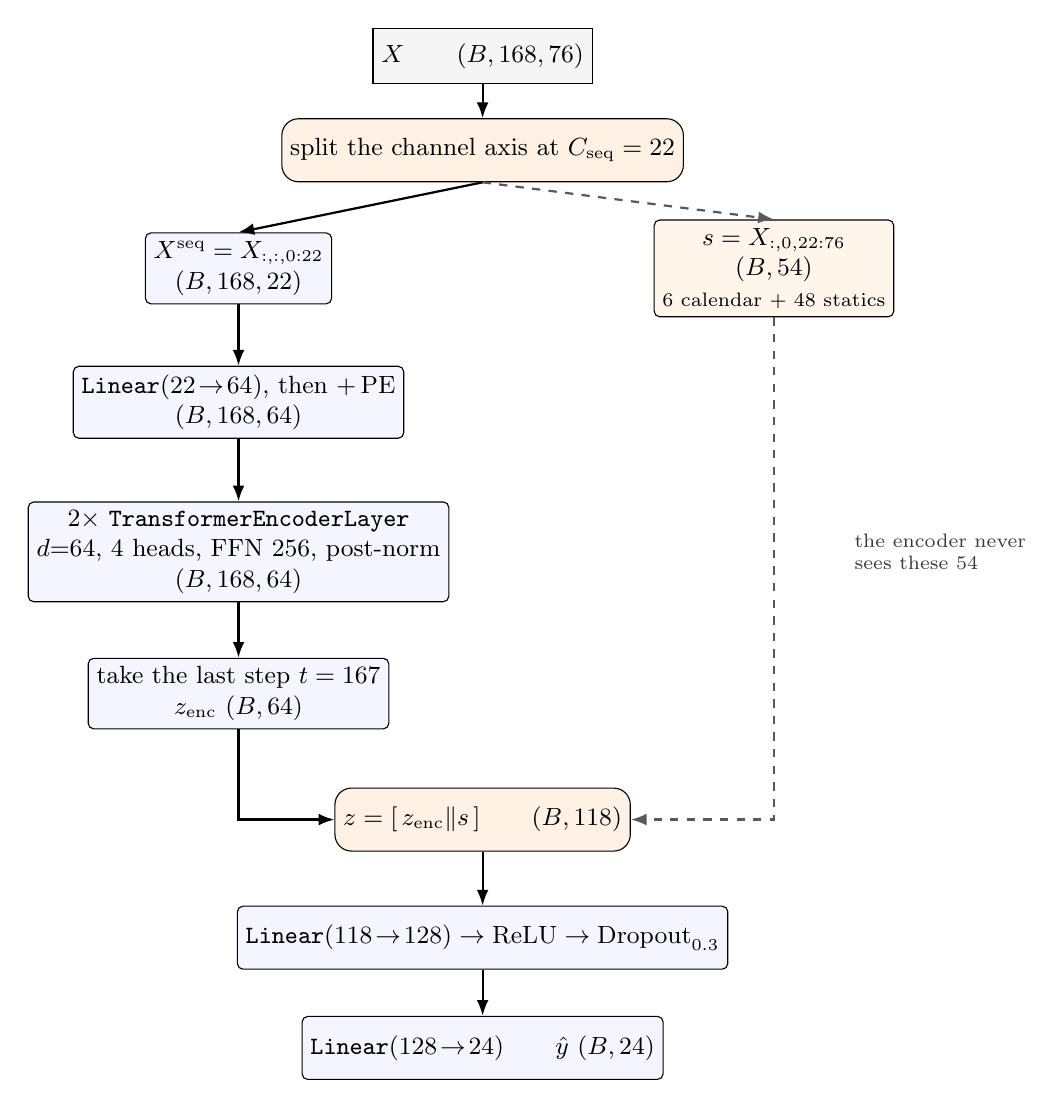
\begin{tikzpicture}[x=1cm,y=1cm]
\node[data] (in)   at (0,0)      {$X$\qquad$(B,168,76)$};
\node[op]   (spl)  at (0,-1.2)   {split the channel axis at $C_{\text{seq}}=22$};
\node[blk]  (seq)  at (-3.1,-2.7) {$X^{\text{seq}} = X_{:,:,0:22}$\\$(B,168,22)$};
\node[blk,fill=orange!8] (sta) at (3.7,-2.7)
      {$s = X_{:,0,22:76}$\\$(B,54)$\\\scriptsize 6 calendar $+$ 48 statics};
\node[blk]  (proj) at (-3.1,-4.4) {\code{Linear}$(22\!\to\!64)$, then $+\,\mathrm{PE}$\\$(B,168,64)$};
\node[blk]  (enc)  at (-3.1,-6.3) {$2\times$ \code{TransformerEncoderLayer}\\
                                   $d{=}64$, 4 heads, FFN $256$, post-norm\\$(B,168,64)$};
\node[blk]  (last) at (-3.1,-8.1) {take the last step $t = 167$\\$z_{\text{enc}}\ (B,64)$};
\node[op]   (cat)  at (0,-9.7)   {$z = [\,z_{\text{enc}} \Vert s\,]$\qquad$(B,118)$};
\node[blk]  (h1)   at (0,-11.2)  {\code{Linear}$(118\!\to\!128) \to \ReLU \to \Drop_{0.3}$};
\node[blk]  (h2)   at (0,-12.6)  {\code{Linear}$(128\!\to\!24)$\qquad$\hat y\ (B,24)$};
\draw[ar]  (in)  -- (spl);
\draw[ar]  (spl.south) -- (seq.north);
\draw[ard] (spl.south) -- (sta.north);
\draw[ar]  (seq)  -- (proj);
\draw[ar]  (proj) -- (enc);
\draw[ar]  (enc)  -- (last);
\draw[ar]  (last.south) |- (cat.west);
\draw[ard] (sta.south)  |- (cat.east);
\draw[ar]  (cat) -- (h1);
\draw[ar]  (h1)  -- (h2);
\node[font=\scriptsize,gray!45!black,align=left,anchor=west] at (4.6,-6.3)
      {the encoder never\\sees these 54};
\end{tikzpicture}}
\caption{Dashed $=$ the static skip. Across arms the head input $z$ is
$110/118/120/128$.}
\end{figure}

\paragraph{One token $=$ one hour.} 168 tokens, each the $\R^{22}$ vector observed
at that hour. No vocabulary, so the ``embedding'' is one learned affine map shared
across positions, $e_t = W_p x_t + b_p$, $W_p \in \R^{64\times22}$. No patching, no
\code{[CLS]}, no padding or mask (every sample has exactly 168 real hours), and the
statics are not tokens --- they are constant in $t$.

\paragraph{Position.} Fixed sinusoidal, \emph{added}:
$\mathrm{PE}_{t,2i} = \sin(t/10000^{2i/64})$, $\mathrm{PE}_{t,2i+1} = \cos(\cdot)$.
It encodes absolute index, not ``3\,pm'' --- the window always ends at midnight, so
clock hour is $t \bmod 24$, and the target day's calendar arrives through the
statics.

\paragraph{Encoder, $\times2$.} Bidirectional (all 168 hours are past), 4 heads,
$d_k = 16$:
\begin{align}
\mathrm{head}_j &= \softmax\!\left(\tfrac{Q_jK_j^{\!\top}}{\sqrt{16}}\right)V_j,
  \qquad \MHA(H) = [\mathrm{head}_1\Vert\cdots\Vert\mathrm{head}_4]W^O, \\
H' &= \LN\big(H + \Drop(\MHA(H))\big), \qquad
H'' = \LN\big(H' + \Drop(\FFN(H'))\big).
\end{align}
Pooling is the last timestep, $z_{\text{enc}} = H''_{:,167,:}$ --- the hour before
the cutoff, and the one position that has attended to every other.

\paragraph{Parameters.} $1472$ (projection) $+\ 99\,968$ (2 encoder layers)
$+\ 18\,328$ (head) $= \mathbf{119\,768}$.

\subsection{LSTM}

Same plumbing, attention replaced by a 2-layer LSTM, hidden 128. \textbf{No input
projection} --- the $\R^{22}$ vector goes straight into the gates, so
$W_{i\bullet}^{(1)} \in \R^{512\times22}$ absorbs the $22\to64$ map. Position is
implicit in the recurrence order.
\[
i_t, f_t, o_t = \sigma(W_{i\bullet}x_t + W_{h\bullet}h_{t-1} + b),
\quad g_t = \tanh(\cdot),
\quad c_t = f_t \odot c_{t-1} + i_t \odot g_t,
\quad h_t = o_t \odot \tanh(c_t).
\]
Trace $(B,168,22) \to (B,168,128) \to (B,128) \xrightarrow{\Vert s} (B,182) \to (B,24)$.
$\mathbf{236\,440}$ parameters --- twice the transformer, and slightly worse.

\subsection{MSTNN}

The idea is the reshape: fold 168 steps so one axis is the day and the other the hour.
\[
X^{\text{seq}} \in \R^{B\times168\times22} \to \R^{B\times7\times24\times22}
\to G \in \R^{B\times\underbrace{22}_{\text{channels}}\times\underbrace{7}_{\text{days}}\times\underbrace{24}_{\text{hours}}}
\]
A $(k_d,k_h)$ kernel then covers $k_d$ consecutive days at the \emph{same clock
hours} --- a receptive field a 1-D conv would need dilation 24 to reach. The unit is
a (day, hour) cell, not a token: no embedding, no positional encoding, adjacency in
both axes is structural. The diurnal and weekly periods the transformer must recover
from sinusoids are built into the layout here.

\begin{figure}[htbp]
\centering
\fitfig{%
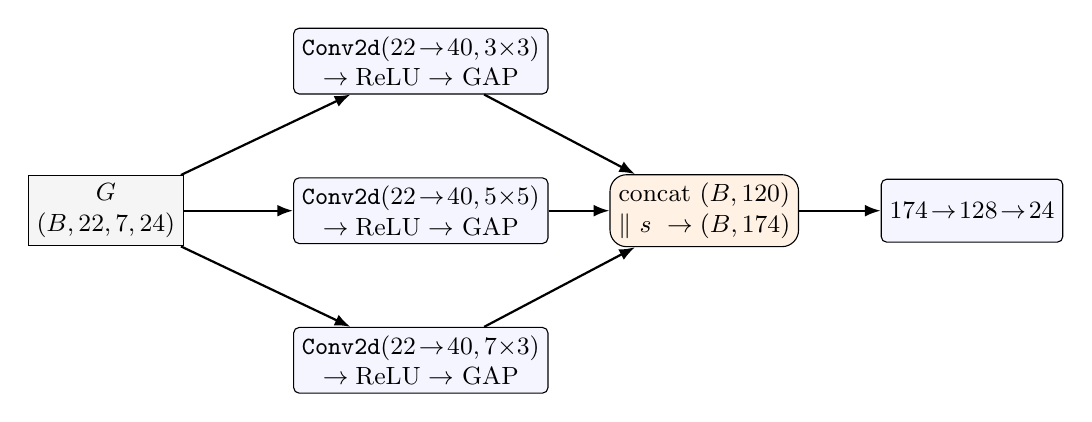
\begin{tikzpicture}[x=1cm,y=1cm]
\node[data] (g)  at (0,0) {$G$\\$(B,22,7,24)$};
\node[blk] (b1) at (4.0,1.9)  {\code{Conv2d}$(22\!\to\!40, 3{\times}3)$\\$\to\ReLU\to$ GAP};
\node[blk] (b2) at (4.0,0)    {\code{Conv2d}$(22\!\to\!40, 5{\times}5)$\\$\to\ReLU\to$ GAP};
\node[blk] (b3) at (4.0,-1.9) {\code{Conv2d}$(22\!\to\!40, 7{\times}3)$\\$\to\ReLU\to$ GAP};
\node[op]  (cc) at (7.6,0)  {concat $(B,120)$\\$\Vert\ s\ \to (B,174)$};
\node[blk] (hd) at (11.0,0) {$174\!\to\!128\!\to\!24$};
\draw[ar] (g) -- (b1); \draw[ar] (g) -- (b2); \draw[ar] (g) -- (b3);
\draw[ar] (b1) -- (cc); \draw[ar] (b2) -- (cc); \draw[ar] (b3) -- (cc);
\draw[ar] (cc) -- (hd);
\end{tikzpicture}}
\caption{Three scales: local ($3{\times}3$), medium ($5{\times}5$), full-week
($7{\times}3$, all seven days at once). GAP $=$ global average pool over the whole
$(7,24)$ grid --- it replaces the original flatten-then-FC, which at ${\sim}1.5$k
samples memorised immediately ($4320$ features into the head instead of $120$).}
\end{figure}

\noindent
$\mathbf{74\,016}$ parameters, the smallest of the neural architectures.

\subsection{Hard-routed MoE head}\label{sec:moe}

Three architectures (\code{moe\_\{transformer,mstnn,lstm\}}) swap the MLP head for
a \code{RegimeHead}: 12 experts, \textbf{no gating network}. Season comes from the
target day's month (per sample); within a season the 24 output hours are partitioned
among three experts (per output index).

\begin{center}\small
\begin{tabular}{@{}llll@{}}
\toprule
Season (months) & \code{low} & \code{peak} & \code{high} \\
\midrule
summer $\{7,8\}$           & 1--6 \hfill(6) & 12--20 \hfill(9)       & 0, 7--11, 21--23 \hfill(9) \\
upper\_shoulder $\{6,9\}$  & 1--6 \hfill(6) & 14--19 \hfill(6)       & 0, 7--13, 20--23 \hfill(12) \\
shoulder $\{3,4,5,10,11\}$ & 0--4 \hfill(5) & 6--9, 17--20 \hfill(8) & 5, 10--16, 21--23 \hfill(11) \\
winter $\{12,1,2\}$        & 0--4 \hfill(5) & 6--9, 17--21 \hfill(9) & 5, 10--16, 22--23 \hfill(10) \\
\bottomrule
\end{tabular}
\end{center}

\noindent
All four seasons are computed, then hard-selected by $\kappa_i$; the unselected
three are sliced away before the loss and get no gradient. Only three of twelve
experts are active per sample.

\subsection{Soft-gated MoE head}\label{sec:smoe}

\code{RegimeHead} partitions the data \emph{and} the output vector. On 1461 training
days its twelve experts see $1\,428$--$7\,018$ target scalars each against $35\,064$
for a single head, and every hard-routed variant loses to its plain counterpart:
$+0.087/+0.103/+0.119$\,pp (transformer/mstnn/lstm, residual) and
$+0.827/+0.649/+1.788$\,pp (direct).

The standard form (Jacobs et al.\ 1991; Shazeer et al.\ 2017) partitions nothing:
\begin{equation}
  \mathbf{g} = \softmax\!\left(W_g\,\mathbf{z}_{\text{gate}} + \boldsymbol\varepsilon\right),
  \qquad
  \hat{\mathbf{y}} = \sum_{i=1}^{N} g_i\,E_i(\mathbf{z}) \in \R^{24},
\end{equation}
$\boldsymbol\varepsilon \sim \mathcal{N}(0,\sigma_g^2)$ on the logits in training only.
Every expert emits all 24 hours and gets gradient from every sample, weighted: a July
day still passes through the ``winter'' expert, at a small weight.

\begin{figure}[htbp]
\centering
\fitfig{
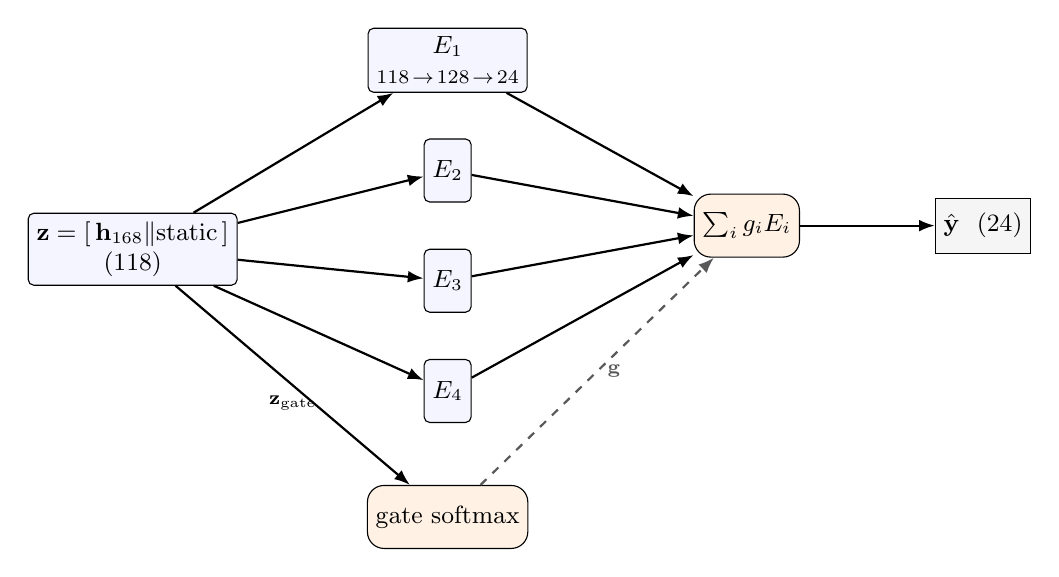
\begin{tikzpicture}[x=1cm,y=1cm]
\node[blk]  (z)  at (0,0) {$\mathbf{z} = [\,\mathbf{h}_{168} \Vert \text{static}\,]$\\$\dims{118}$};
\node[blk] (e1) at (4.0,2.4)  {$E_1$\\\scriptsize $118\!\to\!128\!\to\!24$};
\node[blk] (e2) at (4.0,1.0)  {$E_2$};
\node[blk] (e3) at (4.0,-0.4) {$E_3$};
\node[blk] (e4) at (4.0,-1.8) {$E_4$};
\node[op]  (g)  at (4.0,-3.4) {gate $\softmax$};
\node[op]   (sum) at (7.8,0.3) {$\sum_i g_i E_i$};
\node[data] (y)   at (10.8,0.3) {$\hat{\mathbf{y}}\ \dims{24}$};
\foreach \n in {e1,e2,e3,e4} \draw[ar] (z) -- (\n);
\draw[ar] (z) -- (g) node[midway,below,font=\scriptsize]{$\mathbf{z}_{\text{gate}}$};
\foreach \n in {e1,e2,e3,e4} \draw[ar] (\n) -- (sum);
\draw[ard] (g) -- (sum) node[midway,right,font=\scriptsize]{$\mathbf{g}$};
\draw[ar] (sum) -- (y);
\end{tikzpicture}}
\caption{Encoder unchanged from \S\ref{sec:transformer}; only
$\mathbf{z} \to \hat{\mathbf{y}}$ differs. The gate supplies weights, not a selection.}
\end{figure}

\noindent
\textbf{Load balancing.} A softmax gate collapses if left alone. With
$m_i = \sum_b g_{i,b}$ over a batch,
$\Loss = \Loss_{\text{fc}} + \lambda_{\text{bal}}\big(\mathrm{sd}(\mathbf{m})/\mathrm{mean}(\mathbf{m})\big)^2$,
through the same \code{aux\_loss} hook GARCHFormer uses.

\begin{center}\small
\begin{tabular}{@{}lrrrrl@{}}
\toprule
Variant & Parameters & Experts & Head & Gate in & Gate sees \\
\midrule
\code{transformer}       & 119\,768 & 1 & 128 & --- & --- \\
\code{transformer\_wide} & 170\,104 & 1 & 480 & --- & --- \\
\code{smoe\_z}           & 175\,228 & 4 & 128 & 118 & all of $\mathbf{z}$ \\
\code{smoe\_cal}         & 174\,780 & 4 & 128 & 6   & target-day calendar only \\
\bottomrule
\end{tabular}
\end{center}

\noindent
\code{smoe\_cal}'s gate reads only the 6 calendar channels --- the softened form of
\code{RegimeHead}'s month rule, with learned boundaries and no sample excluded from
any expert. The two mixtures differ by $(118-6)\times4 = 448$ parameters, the gate
matrix alone. \code{transformer\_wide} is a \emph{control}: the mixtures carry
${\sim}55$k extra parameters, so beating \code{transformer} alone could be capacity
rather than mixing.

\noindent
\textbf{Read the gate, not the MAPE.} Mean $\approx 1/N$ with a \emph{high}
per-sample max means the gate routes decisively but to a different expert each day
--- the outcome the design bets on. Both flat means no routing happened, which is a
result: a soft mixture that declines to specialise degenerates to an average of its
experts, not to under-trained specialists. One mean $>0.85$ is collapse. Expert
identity is arbitrary up to permutation, so gates are read from one seed, never
averaged.

\subsection{GARCHFormer (ARCHFormer3)}\label{sec:garchformer}

Moyi Guo's \code{archformer3}, vendored: \code{layers.py} byte-identical,
\code{pointmodels.py} one import line changed. Written here: the adapter giving it
this repo's \code{train/predict/evaluate} signatures, plus a hook for its auxiliary
loss. Everything else is shared with the other eight --- same tensor, split,
embargo, scalers, evaluator.

\paragraph{One token $=$ one day.} \code{patch\_len}$=24$, so $168/24 = 7$ tokens and
every attention matrix is $7\times7$. That is what makes the GARCH recursion
affordable: it is a Python loop that runs seven times. All $C$ channels go in ---
there is no static skip, so the 54 constants are presented 24 times inside each
patch. Upstream's design, kept.

\begin{figure}[htbp]
\centering
\fitfig{%
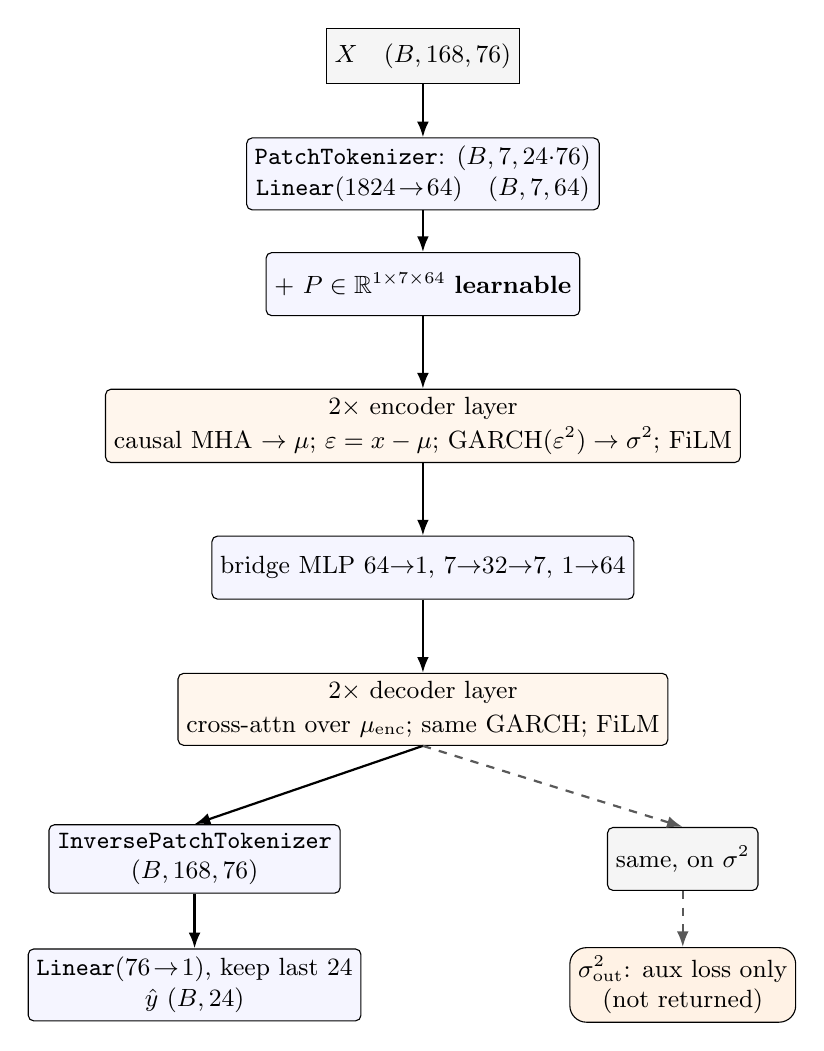
\begin{tikzpicture}[x=1cm,y=1cm]
\node[data] (in)  at (0,0)     {$X$\quad$(B,168,76)$};
\node[blk]  (tok) at (0,-1.5)  {\code{PatchTokenizer}: $(B,7,24{\cdot}76)$\\
                                \code{Linear}$(1824\!\to\!64)$\quad$(B,7,64)$};
\node[blk]  (pe)  at (0,-2.9)  {$+\ P \in \R^{1\times7\times64}$ \textbf{learnable}};
\node[blk,fill=orange!7] (enc) at (0,-4.7)
      {$2\times$ encoder layer\\[1pt]
       causal MHA $\to \mu$;\ $\varepsilon = x-\mu$;\ GARCH$(\varepsilon^2) \to \sigma^2$;\ FiLM};
\node[blk]  (br)  at (0,-6.5)  {bridge MLP $64{\to}1$, $7{\to}32{\to}7$, $1{\to}64$};
\node[blk,fill=orange!7] (dec) at (0,-8.3)
      {$2\times$ decoder layer\\[1pt]
       cross-attn over $\mu_{\text{enc}}$;\ same GARCH;\ FiLM};
\node[blk]  (inv) at (-2.9,-10.2) {\code{InversePatchTokenizer}\\$(B,168,76)$};
\node[blk,fill=gray!8] (invs) at (3.3,-10.2) {same, on $\sigma^2$};
\node[blk]  (hd)  at (-2.9,-11.8) {\code{Linear}$(76\!\to\!1)$, keep last 24\\$\hat y\ (B,24)$};
\node[op]   (aux) at (3.3,-11.8) {$\sigma^2_{\text{out}}$: aux loss only\\(not returned)};
\draw[ar] (in) -- (tok);  \draw[ar] (tok) -- (pe);   \draw[ar] (pe) -- (enc);
\draw[ar] (enc) -- (br);  \draw[ar] (br) -- (dec);
\draw[ar] (dec.south) -- (inv.north);
\draw[ard] (dec.south) -- (invs.north);
\draw[ar] (inv) -- (hd);  \draw[ard] (invs) -- (aux);
\end{tikzpicture}}
\caption{Sequence length is $7$, not $168$, everywhere between the tokenizer and its
inverse. The grey column is the variance path: computed every forward pass,
supervises training, then discarded.}
\end{figure}

\paragraph{Mean path.} Causal MHA over the 7 day-tokens --- day $t$ attends only to
$\le t$. Opposite to \S\ref{sec:transformer}, where attention is bidirectional. Both
are legitimate (all 168 hours are past); the causal form is what makes the residual
below a genuine one-step-ahead innovation rather than a smoothed fit.

\paragraph{Variance path --- the GARCH block.} The innovation is available without a
second pass, $\varepsilon = x - \mu$. A causal attention first forms a
data-dependent weighting of past squared innovations,
$a_t = \sum_{j \le t}\tilde A_{tj}\,\varepsilon^2_j$ --- an ARCH term with learned
lag weights instead of fixed ones. Then a per-channel GARCH$(1,1)$ recursion over
the 7 tokens:
\begin{equation}
  \sigma^2_t = \omega + \alpha \odot a_t + \beta \odot \sigma^2_{t-1},
  \qquad \sigma^2_0 = \mathbf{0},\quad t = 1,\ldots,7,
\end{equation}
\begin{equation}
  \omega = \mathrm{softplus}(\omega_{\text{raw}}),
  \quad \alpha = \sigma(\alpha_{\text{raw}}) \in (0,1),
  \quad \beta = \frac{\sigma(\beta_{\text{raw}})}{\max\big(\alpha + \sigma(\beta_{\text{raw}}),\,1\big)} .
\end{equation}
That denominator is exactly the covariance-stationarity condition
$\alpha + \beta \le 1$, imposed by construction rather than by a penalty, so the
recursion cannot diverge. $\omega,\alpha,\beta \in \R^{64}$ --- 64 independent GARCH
processes, one per embedding channel.

\paragraph{FiLM fusion.} The variance modulates the mean path:
$[\gamma \Vert \beta_f] = W_{f2}\,\mathrm{GELU}(W_{f1}\,\mathrm{softplus}(W_r\sigma^2))$,
then $h = \LN(\gamma \odot \mu + \beta_f)$ and $x_{\text{next}} = \LN(x + h)$. A
channel whose recent innovations were large gets its mean-path activation rescaled
--- the mechanism by which a variance model changes a \emph{point} forecast.

\paragraph{Output.} The model reconstructs the \emph{entire} input grid
($168 \times 76$) and reads the forecast off the last 24 positions through one
shared $76\to1$ projection. The forecast head is therefore tied to a reconstruction
task, which is why the inverse tokenizer is the second-largest block.

\paragraph{Loss.} MSE (upstream's, not this repo's Huber) plus a variance-consistency
term through the \code{aux\_loss} hook:
\begin{equation}
  \Loss = \tfrac{1}{24B}\textstyle\sum_{i,h}(\hat y_{i,h}-y_{i,h})^2
  \;+\; \lambda\,\tfrac{1}{24B}\textstyle\sum_{i,h}
  \big|\sigma^2_{\text{out},i,h} - (y_{i,h}-\hat y_{i,h})^2\big|,
  \qquad \lambda = 0.1 .
\end{equation}
Not detached, so it also pushes the mean path. $\lambda = 0$ recovers ARCHFormer2 on
identical weights. $\sigma^2$ is an auxiliary target, never an output ---
\code{predict()} returns $\hat y$ alone.

\begin{center}\small
\begin{tabular}{@{}lrr@{}}
\toprule
Component & Parameters & Share \\
\midrule
\code{PatchTokenizer} $(1824 \to 64)$        & 116\,800 & 23.1\,\% \\
\code{ARCHEncoder} $2\times$                 & 167\,296 & 33.1\,\% \\
bridge                                       & \phantom{000}680 & \phantom{0}0.1\,\% \\
\code{ARCHDecoder} $2\times$                 & 100\,864 & 20.0\,\% \\
\code{InversePatchTokenizer} $(64 \to 1824)$ & 118\,560 & 23.5\,\% \\
head $(76 \to 1)$ $+$ learnable PE           & \phantom{00}\,525 & \phantom{0}0.1\,\% \\
\midrule
\textbf{Total} (\code{\_cong})               & \textbf{504\,725} & \\
\bottomrule
\end{tabular}
\end{center}

\noindent
Nearly half sits in the two patch projections, both of which scale with $C$ ---
$479\,949$ on the base arm, $544\,986$ on \code{\_cong\_lmp}. Largest of the nine.
Hyperparameters ($d{=}64$, 4 heads, $2{+}2$ layers, \code{patch\_len} 24, MSE,
lr $2{\cdot}10^{-3}$, 50 epochs) are all his; the best-validation checkpoint is this
repo's addition --- his trainer computes it but leaves the save commented out.

\subsection{Residual variants}\label{sec:resid}

Nine of the eighteen. \textbf{Nothing changes but the target.} The baseline is the
sample's own same-hour-last-week mean of preliminary load, in raw MW:
\begin{equation}
  b_{i,h} = \frac17\sum_{j=0}^{6}\tilde x_{i,\,h+24j},
  \qquad h = 0,\ldots,23 ,
\end{equation}
the window ending at a midnight cutoff so position $k$ sits at clock hour
$k \bmod 24$. Train on $\tilde r_{i,h} = (y^{\text{MW}}_{i,h} - b_{i,h} - \mu_r)/\sigma_r$,
predict $\hat y^{\text{MW}}_{i,h} = \sigma_r \hat{\tilde r}_{i,h} + \mu_r + b_{i,h}$,
then re-standardise so the caller's usual inverse cancels it exactly and the
residual plumbing is invisible downstream.

\noindent
Legitimate because it is computed from the sample's \emph{own} lookback (nothing fit
on the training set, so no leakage) and reads only preliminary load (published in
real time, so it deploys on the same path). $(\mu_r,\sigma_r)$ and the baseline mode
are saved beside the weights.

\noindent
A residual model outputting zero reproduces the baseline, so the baseline's own
score is a hard floor: $7.72\%$ on dom, $10.40\%$ on bge. Every residual variant
beats its own direct counterpart, on both zones.

\subsection{Seed ensembling}\label{sec:seedens}

\code{\_seq\_trainer.py} never calls \code{torch.manual\_seed}, so every
sequence-model row in the scoreboard is one undocumented draw. How wide depends on
the architecture (dom, \code{\_cong}, residual):

\begin{center}\small
\begin{tabular}{@{}lrrrl@{}}
\toprule
Model & seeds & mean & sd & range \\
\midrule
\code{archformer\_hp\_residual}  & 5 & 3.274 & 0.115 & 3.103--3.415 \\
\code{archformer\_residual}      & 5 & 3.569 & 0.151 & 3.408--3.728 \\
\code{transformer\_residual}     & 4 & 3.065 & 0.029 & 3.022--3.093 \\
\bottomrule
\end{tabular}
\end{center}

\noindent
GARCHFormer's spread is $4\times$ the transformer's ($504\,725$ parameters over
$1461$ days) and exceeds the $0.22$\,pp gap between them, so single-seed rankings
between the two are not decidable.

\noindent
The \emph{seed mean} averages five MAPE values. The \emph{ensemble} averages the
five predictions into one model, $\bar{\mathbf{y}}_d = \frac1K\sum_k \hat{\mathbf{y}}^{(k)}_d$,
$K = 5$, and scores it once. By the triangle inequality it can never be worse:
\begin{equation}
  \mathrm{MAPE}(\bar{\mathbf{y}}) \;\le\; \tfrac1K\textstyle\sum_k \mathrm{MAPE}(\hat{\mathbf{y}}^{(k)}),
\end{equation}
and likewise for peak MAPE --- the question is only how much, which scales with how
uncorrelated the members' errors are.

\begin{center}\small
\begin{tabular}{@{}llrrr@{}}
\toprule
Zone & Variant & seed mean & ensemble & gain \\
\midrule
dom & \code{archformer\_hp\_residual} & 3.274 & \textbf{2.987} & $0.287$ \\
dom & \code{archformer\_residual}     & 3.569 & 3.219 & $0.350$ \\
dom & \code{archformer\_hp}           & 3.965 & 3.734 & $0.231$ \\
dom & \code{archformer}               & 4.313 & 4.023 & $0.290$ \\
bge & \code{archformer\_hp\_residual} & 4.798 & 4.476 & $0.322$ \\
bge & \code{archformer\_residual}     & 4.878 & 4.527 & $0.351$ \\
bge & \code{archformer\_hp}           & 4.619 & 4.287 & $0.332$ \\
bge & \code{archformer}               & 5.290 & 4.690 & $0.600$ \\
\bottomrule
\end{tabular}
\end{center}

\noindent
The gain is large \emph{because} the seed variance is large. dom's $2.987$ is below
every single-seed \code{transformer\_residual} run (best $3.022$, mean $3.065$), and
its peak MAPE $3.326$ is the best of any model. At the single-model level the
transformer is still better --- $3.065$ lies outside GARCHFormer's 95\% CI
$[3.131, 3.417]$ --- so the ensemble, not the network, closes the gap.

\noindent
\textbf{Not the best seed.} Reporting the lowest of five test scores is selection on
the test set. Only the mean with its spread (describes the architecture, not a
deployable model) or the ensemble (a fixed model using no test information) is
defensible. \textbf{Independent of checkpoint choice}: across the shipped early
stopping and fixed 20- and 30-epoch budgets the seed sd is $0.115/0.145/0.098$ with
no ordering. Removing early stopping separately costs $0.15$\,pp.

% =====================================================================
\section{Probabilistic baselines}
% =====================================================================

Four, each reproducing one IEEE TSG paper, scored on 99 percentiles. Structurally
isolated: each reads only the cleaned hourly CSV, and rows are \emph{hours}, not the
per-day samples above.

\begin{center}\small
\begin{tabular}{@{}llp{6.2cm}r@{}}
\toprule
Paper & Mechanism & Core & dom pinball \\
\midrule
Xie \& Hong (2018) & temperature scenarios $\to$ MLR
  & 285-column MLR (Day$\times$Hour, Month, Month/Hour-interacted cubic in
    standardised $T$); 30 past weather years $\times$ date shifts give $J$ scenarios;
    quantiles are the empirical percentiles of the $J$ point forecasts & 432.10 \\
\addlinespace
Liu et al.\ (2017) & sister forecasts $\to$ QRA
  & 8 sisters $=$ 2 estimation windows $\times$ 4 selection schemes, differing in a
    temperature recency block; per day and per level,
    $\min_\beta \sum \rho_p(\ln y - \beta_0 - \sum_i \beta_i \ln f^{(i)})$ by Koenker
    IRLS, then sorted & \textbf{177.26} \\
\addlinespace
Zhang et al.\ (2019) & one net, 99 outputs
  & $101 \to 500 \to 500 \to 99$, PReLU, dropout 0.5, Gaussian noise $0.3$, summed
    pinball; pool $1645 \to 100{+}3$ by RFE. $352\,099$ parameters & 250.52 \\
\addlinespace
Li et al.\ (2020) & 15 densities $\to$ CRPS-weighted GMM
  & 5 GPR $+$ 5 QRNN $+$ 5 QRGB; deciles $\to$ $(\mu,\sigma)$ by probit OLS; weights
    from $\min_w w^{\!\top}Qw + c^{\!\top}w$ on the simplex, closed-form mixture CRPS
    (Baringhaus--Franz), so $w_i = 0$ drops a model & 483.06 \\
\bottomrule
\end{tabular}
\end{center}

\noindent
\textbf{Horizons are not identical.} QRA issues at $D{-}1$ for day $D$; the other
three, and all eighteen point models, issue at $D{-}1$ for day $D{+}1$. QRA's winning
$177.3$ is therefore not directly comparable with QRNN's $250.5$.

\noindent
\textbf{Metrics.} Pinball $\mathrm{PB}_q$ averaged over 99 levels; Winkler
$W_c = \delta + \frac{2}{\alpha}(L-y)\ind\{y<L\} + \frac{2}{\alpha}(y-U)\ind\{y>U\}$
with $\delta = U-L$; CRPS $= 2\int_0^1 \mathrm{PB}_\tau d\tau$; coverage. Winkler is
carried because pinball alone cannot separate ``covers everything because it is
enormous'' from ``covers everything and is tight''.

% =====================================================================
\section{Results}
% =====================================================================

\noindent
Point metrics: MAPE, MAE, RMSE, ME as usual, plus \textbf{peak MAPE} (restricted to
the top decile of true load) and \textbf{BRS}, the OLS slope of per-bin mean error on
per-bin mean load over ten equal-count load bins. BRS $>0$ over-predicts at peak,
$<0$ under-predicts. \emph{Every} model here has BRS $<0$ --- they all shave the peak.

\begin{center}\small
\begin{tabular}{@{}llrrrrr@{}}
\toprule
\multicolumn{7}{@{}l}{\textbf{dom} --- 313 test days, 2025-10-17 to 2026-08-25} \\
\midrule
Model & Best arm & MAPE\,\% & MAE & RMSE & peak\,\% & BRS \\
\midrule
\code{transformer\_residual}      & \code{\_cong} & \textbf{3.018} & 504.8 & 687.1 & 3.937 & $-0.0553$ \\
\code{mstnn\_residual}            & \code{\_cong} & 3.042 & 514.0 & 698.3 & 4.444 & $-0.0845$ \\
\code{moe\_transformer\_residual} & \code{\_cong} & 3.105 & 521.5 & 703.6 & 4.113 & $-0.0555$ \\
\code{lstm\_residual}             & \code{\_cong\_lmp} & 3.127 & 521.4 & 707.6 & 4.073 & $-0.0573$ \\
\code{archformer\_residual}       & \code{\_cong} & 3.263 & 542.7 & 726.6 & \textbf{3.855} & $\mathbf{-0.0198}$ \\
\code{xgboost\_residual}          & \code{\_cong} & 3.300 & 551.9 & 748.0 & 4.296 & $-0.0707$ \\
\code{transformer}                & \code{''}     & 3.438 & 577.5 & 760.5 & 4.920 & $-0.1061$ \\
\code{archformer}                 & \code{\_cong} & 3.603 & 611.1 & 827.0 & 5.948 & $-0.1029$ \\
\code{xgboost}                    & \code{\_cong} & 4.860 & 840.8 & 1149.3 & 8.621 & $-0.1857$ \\
\midrule
\multicolumn{2}{@{}l}{\emph{naive same-hour-last-week}} & 7.72 & 1280.4 & 1682.8 & --- & --- \\
\multicolumn{2}{@{}l}{\emph{TimesFM 3.0, zero-shot}}    & 5.242 & 872.6 & 1208.0 & 5.835 & $-0.0598$ \\
\bottomrule
\end{tabular}
\end{center}

\noindent
\textbf{GARCHFormer's result.} Mid-pack on MAPE (23rd of 66 runs) but first on
\emph{both} peak MAPE ($3.855$) and $|$BRS$|$ ($-0.0198$, against a previous best of
$-0.0305$ and $-0.0553$ for the model that beats it on MAPE). That is what the
architecture predicts: load volatility is highest at the peak, the GARCH recursion
gives an explicit per-channel estimate of it, and FiLM lets the network rescale the
mean path accordingly. A model that can represent ``this hour is high-variance'' has
a mechanism for not regressing the peak toward the mean.

\noindent
\textbf{Feature arms.} Congestion is a consistent small gain ($-0.4$ to $-2.0\%$
relative); the price block is a consistent \emph{loss} on dom in both forms, despite
a LightGBM gain breakdown putting the ten DA price statics at $25.35\%$ of training
gain. High training gain with worse test error is what an over-trusted proxy looks
like: price is a downstream consequence of load, so it correlates hard in sample
while carrying supply-side noise, and its elasticity to load drifts by ${>}2\times$
across the record.

\begin{center}\small
\begin{tabular}{@{}lrrrr@{}}
\toprule
& \multicolumn{4}{c}{dom MAPE\,\% by arm} \\
\cmidrule(l){2-5}
Model & \code{''} & \code{\_cong} & \code{\_lmp} & \code{\_cong\_lmp} \\
\midrule
\code{transformer\_residual} & 3.159 & \textbf{3.018} & 3.089 & 3.148 \\
\code{mstnn\_residual}       & 3.068 & \textbf{3.042} & 3.123 & 3.049 \\
\code{xgboost\_residual}     & 3.313 & \textbf{3.300} & 3.435 & 3.427 \\
\code{lightgbm\_residual}    & 3.532 & \textbf{3.462} & 3.547 & 3.540 \\
\bottomrule
\end{tabular}
\end{center}

\noindent
\textbf{bge} is the harder zone ($\approx$3\,GW against dom's $\approx$17\,GW, and
its preliminary-load proxy is the MIDATL regional aggregate divided by $8.8$, which
carries a $3.3\%$ shape mismatch no rescaling removes). Best there:
\code{transformer\_residual} $4.434\%$, \code{mstnn\_residual} $4.458\%$, TimesFM
$7.416\%$.

\begin{center}\small
\begin{tabular}{@{}lrrrrl@{}}
\toprule
Probabilistic (dom) & pinball & Winkler-50 & Winkler-90 & CRPS & horizon \\
\midrule
QRA ($m{=}8$, $L{=}183$)        & \textbf{177.26} & \textbf{1571.3} & \textbf{2826.8} & 355.4 & $D{-}1 \to D$ \\
iQRNN-500-ZD                    & 250.52 & 2220.6 & 4586.9 & 495.2 & $D{-}1 \to D{+}1$ \\
bQRNN-400 \emph{(control)}      & 404.23 & 3333.0 & 14197.2 & 794.4 & $D{-}1 \to D{+}1$ \\
Scenario MLR $(20,10)$          & 432.10 & 3827.1 & 6962.1 & --- & weather-driven \\
Density, best member (XGB4)     & 469.05 & 4188.4 & 7812.8 & 929.1 & $D{-}1 \to D{+}1$ \\
Density, CRPS-guided            & 483.96 & 4312.9 & 7933.3 & 958.5 & $D{-}1 \to D{+}1$ \\
\bottomrule
\end{tabular}
\end{center}

\noindent
Only QRA is close to nominal coverage ($86.8\%$ at nominal $90\%$). The QRNN family
is miscalibrated in one direction; the scenario ensemble is far too narrow at every
level, which is structural --- its width comes only from temperature spread and
carries no model error. The density combination does \emph{not} beat its own best
member here, consistent with $T_3$ being 56 days against the paper's longer
weight-optimisation window.

\end{document}
